\subsection{多面角}\label{subsec:3-1}

相邻的两面墙壁和天花板所成的屋角,一些塔的塔顶都给我们以多面角的形象。

有公共端点并且不在同一平面内的几条射线,以及相邻两条射线间的平面部分所组成的图形,叫做\zhongdian{多面角}。

如图 \ref{fig:ltjh-3-1}、\ref{fig:ltjh-3-2},都是多面角。 组成多面角的射线 $SA$、$SB$、… 叫做\zhongdian{多面角的棱},
这些射线的公共端点 $S$ 叫做\zhongdian{多面角的顶点},相邻两棱间的平面部分叫做\zhongdian{多面角的面},
相邻两棱组成的角 $\angle ASB$、$\angle BSC$、… 叫做\zhongdian{多面角的面角},
相邻两个面组成的二面角 $E{-}SA{-}B$、$A{-}SB{-}C$、… 叫做\zhongdian{多面角的二面角}。

\begin{figure}[htbp]
    \centering
    \begin{minipage}[b]{7cm}
        \centering
        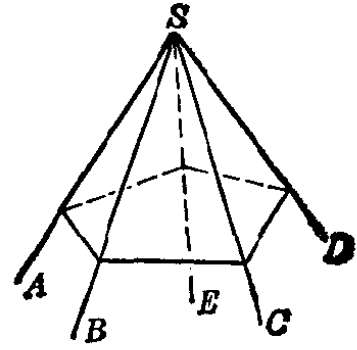
\includegraphics[width=5cm]{../pic/ltjh-ch3-01.png}
        \caption{}\label{fig:ltjh-3-1}
    \end{minipage}
    \qquad \qquad
    \begin{minipage}[b]{7cm}
        \centering
        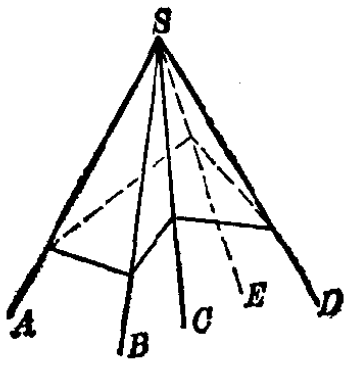
\includegraphics[width=5cm]{../pic/ltjh-ch3-02.png}
        \caption{}\label{fig:ltjh-3-2}
    \end{minipage}
\end{figure}

一个多面角的面数等于它的棱数、面角数、二面角数。多面角最少应有三个面。
多面角依照它的面数分别叫做三面角、四面角、五面角、 … 。

多面角可用表示它的顶点和棱的字母来表示,如图 \ref{fig:ltjh-3-1} 中的多面角记作多面角 $S{-}ABCDE$;
有时也用表示顶点的一个字母表示,记作多面角 $S$。

将多面角的任何一个面伸展成为平面,如果其他各面都在这个平面的同侧,这样的多面角叫做\zhongdian{凸多面角}。
图 \ref{fig:ltjh-3-1} 中的多面角就是一个凸多面角,图 \ref{fig:ltjh-3-2} 中的多面角不是凸多面角。

用一个平面截凸多面角的所有面和棱,一定得到一个凸多边形,如图 \ref{fig:ltjh-3-1}。
用平面截图 \ref{fig:ltjh-3-2} 中的多面角就不能得到凸多边形。

本章只研究凸多面角。凸多面角中,最简单的是三面角。
三个面角都是直角的三面角叫做\zhongdian{直三面角}。 例如屋角、箱角、砖角,都给我们以直三面角的形象。

直三面角 $O{-}XYZ$ 的一般画法如图 \ref{fig:ltjh-3-3}。


\liti[0] 求证:直三面角的各个二面角都是直二面角。

已知:直三面角 $O{-}XYZ$(图 \ref{fig:ltjh-3-3})。

求证:二面角 $\beta{-}OX{-}\gamma$、$\gamma{-}OY{-}\alpha$、$\alpha{-}OZ{-}\beta$ 都是直二面角。

\begin{wrapfigure}[6]{r}{4.5cm}
    \centering
    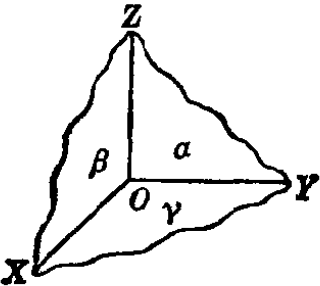
\includegraphics[width=4cm]{../pic/ltjh-ch3-03.png}
    \caption{}\label{fig:ltjh-3-3}
\end{wrapfigure}

\zhengming $\because$ \quad $O{-}XYZ$ 是直三面角,

$\therefore$ \quad \begin{zmtblr}[t]{}
    $\angle XOY = \angle YOZ = \angle ZOX = Rt \angle$, \\
    $OZ \perp OX$, $OY \perp OX$。
\end{zmtblr}

$\therefore$ \quad $\angle YOZ$ 是二面角 $\beta{-}OX{-}\gamma$ 的平面角。

$\because$ \quad $\angle YOZ = Rt \angle$,

$\therefore$ \quad 二面角 $\beta{-}OX{-}\gamma$ 是直二面角。

同理 \quad $\gamma{-}OY{-}\alpha$、$\alpha{-}OZ{-}\beta$ 也是直二面角。


\begin{lianxi}

\xiaoti{二面角是不是多面角?多面角是不是棱锥?它们各有什么区别和联系?}

\xiaoti{求证:三个二面角都是直二面角的三面角是直三面角。}

\end{lianxi}

